\documentclass[tikz]{standalone}
\usepackage{tikz}
\usetikzlibrary{positioning, graphs}
\usetikzlibrary{graphs.standard}
\begin{document}
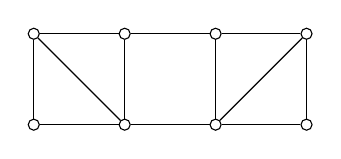
\begin{tikzpicture}
	[vertex/.style={draw,circle,inner sep = 0mm, minimum size = 0.4em},
	 edgelabel/.style = {fill = white, inner sep = 0mm, font=\tiny}]
	\node[vertex] (a) at (0,0) {};
	\node[vertex] [right = of a] (b) {};
	\node[vertex] [right = of b] (c) {};
	\node[vertex] [right = of c] (d) {};
	\node[vertex] [below = of a] (e) {};
	\node[vertex] [right = of e] (f) {};
	\node[vertex] [right = of f] (g) {};
	\node[vertex] [right = of g] (h) {};
	
	\draw (a) -- (b);
	\draw (a) -- (e);
	\draw (a) -- (f);
	\draw (b) -- (c);
	\draw (b) -- (f);
	\draw (c) -- (d);
	\draw (c) -- (g);
	\draw (d) -- (g);
	\draw (d) -- (h);
	\draw (e) -- (f);
	\draw (f) -- (g);
	\draw (g) -- (h);
\end{tikzpicture}
\end{document}